% Define the scope, extend, and how of the study
\chapter{Methodology}
\label{chap:methodology}

This chapter elaborates upon the methodology used in this study. 
The overall structure of what elements this methodology precisely consists of is presented, and how these elements came to be. 
The chapter continues with four sections, each explaining one of these components.
But first, I wish to clarify the nature in which this study is conducted. 

\subsection*{Nature}
The methodology of this study can be characterized as practical as opposed to theoretical, wholistic instead of specific, and iterative compared to linear. The prior works on browser-based geocomputation and geo-vpls indicate that a strong theoretical framework for a \ac{geo-web-vpl} is in place (Source). 
But, and this is especially evident in the prior studies regarding \ac{bbg} (Source), the practical implementation of these theories were only partially successful, and limited in scope. 
This necessitates a practical, wholistic approach in response. 
And, due to the investigative nature of this study, the methodology requires to iterate upon itself, instead of following a singular, linear path. 

% ...
% % Theorie: is er maar je geloofde het niet
% % praktische implementatie om de Throerie weerleggen
% The prior works on browser-based geoprocessing indicate that a theoretical framework for browser-based geoprocessing vpl is in place. 
% But, and this is especially evident in the studies regarding client-side geoprocessing, the practical implementation of these theories

% Choices: 
% - practical > theoretical : Literature study indicates enough theoretical soundness, but lots of practical questions remaining. We wish to  immediate pick up where these studies have left, and therefore we choose the direct, practical study of designing and implementing a prototype application. 
% - wholistic > specific    : Research in one sub-domain could have been more exhaustive in one of the specific sub-studies, instead of covering the full scope it does now. However, This would have been incomplete. What we do now is cover the full pipeline of using a geocomputation library: from creation to web export, to web import, to web utilization. by doing this, we can identify issues caused in one of these
% - iterative > linear      : Given this vast scope, many questions can come up from different angles. The study has to be dynamic to adapt to these demands. 

\subsection*{Structure}
  
\emph{The content of this methodology is based upon the main and supporting research questions. 
As such, it bears fruit to explain how these specific questions were chosen.}

% FIX THISSS 
The related studies in \refchap{chap:related} show that a \ac{geo-web-vpl} as described by this study does not exist yet. However, many examples of geo-vpls (\refsec{sec:related-geovpl}) and web-vpls \refsec{sec:related-webvpl} do exist. 
Based on this, it can be assumed that creating a visual programming environment in a web-browser must be possible. 
Using a \ac*{vpl} for geocomputation must also be possible. 

However, the absence of a geo-web-vpl indicates some sort of hinder, preventing this type of application to be realized. Either geo-VPLs were not able to be properly used in a browser, or web-based VPLs were unable to support geocomputation functionalities. 
Assuming, of course, that researchers and developers of these environments would have wanted to work towards a \ac{geo-web-vpl}.

This study starts from the second assumption: 
Apparently, web-based VPLs are unable to support existing geocomputation functionalities. 
This could be because of several reasons, of which this study identifies four major ones.

geocomputation functionalities might not be able to be properly:
\begin{itemize}[-]
  \item \textbf{compiled} into a format functional on the web
  \item \textbf{loaded} within a web-based VPL
  \item \textbf{facilitated} by the interface of a web-based VPL
  \item \textbf{used} within a web-based VPL
\end{itemize}
As it is unknown which one of these reasons ( or which combination of reasons ) is causing this barrier, the study must encompass all four of these possible hindrances, and access to what extend these aspects form a hinder towards the main goal of a \ac{geo-web-vpl}. 
Moreover, the real reason might not lie in one of these areas, but in the interplay between all of these factors. 

It is this study's objective to pose a solution to this barrier. This is stated by the main research question: \myMainRQ 

The study goes about doing so, by developing a prototype \ac{geo-web-vpl}. 
This prototype is used as an experiment and staging ground to discover the extend of possible hindrances. 
During its development, each one of these four possible hindrances has to be accounted for. 
Per hindrance, document design considerations, and run experiments, all to test to what extend this prototype \ac{geo-web-vpl} fails or succeeds to provide for this aspect. 
After this is done, we can compile a final conclusion to the main research question. 

The methodology of this study is structured to facilitate this process. 
It is subdivided into four components, each representing a sub-research question, which is in turn based upon one of these possible hindrances. The questions are posed in such a way that answering them will require us to explore the extend of the hindrance, and find possible solutions.

The remained of this chapter covers the four components of this methodology, and how this relates to this prototype. 

\begin{note}
TODO: diagram: 4 research questions -> four possible barriers of geocomputation
\end{note}

\begin{note}
TODO: diagram: show the 'locations' of the four research questions ( client / server / native, etc.)
\end{note}

%%%%%%%%%%%%%%%%%%%%%%%%%%%%%%%%%%%%%%%%%%%%%%%%%%%%%%%%%%%%%%%%%%%%%%%%%%%%%%%%%%%%%%%%%%%%%%%%%%%%%%%%%%%%%%
%%%%%%%%%%%%%%%%%%%%%%%%%%%%%%%%%%%%%%%%%%%%%%%%%%%%%%%%%%%%%%%%%%%%%%%%%%%%%%%%%%%%%%%%%%%%%%%%%%%%%%%%%%%%%%
%%%%%%%%%%%%%%%%%%%%%%%%%%%%%%%%%%%%%%%%%%%%%%%%%%%%%%%%%%%%%%%%%%%%%%%%%%%%%%%%%%%%%%%%%%%%%%%%%%%%%%%%%%%%%%
%%%%%%%%%%%%%%%%%%%%%%%%%%%%%%%%%%%%%%%%%%%%%%%%%%%%%%%%%%%%%%%%%%%%%%%%%%%%%%%%%%%%%%%%%%%%%%%%%%%%%%%%%%%%%%
%%%%%%%%%%%%%%%%%%%%%%%%%%%%%%%%%%%%%%%%%%%%%%%%%%%%%%%%%%%%%%%%%%%%%%%%%%%%%%%%%%%%%%%%%%%%%%%%%%%%%%%%%%%%%%

\section{\mySubRQOneTitle} 
\label{sec:method-one}

The first component of the methodology involved the creation of the core of the prototype application, encompassed by the supporting research question : \mySubRQOne

\subsection*{Why}

Before exploring how lifting \emph{existing} geo-computation to the web might take place, this study first wished to discover to what extend the web browser is able to facilitate the interface of a 3D vpl in general.
A 3D VPL is defined as a vpl meant for generic 3D geometry processing.

\subsection*{How}

The method to answer this question is defined as follows. 
The above question of \mySubRQOneTitle is further subdivided into 4 follow-up questions:
\begin{enumerate}[A]
  \item \emph{What are the requirements of a 3D VPL?}
  \item \emph{What can be defined as 'core browser features'?}
  \item \emph{Per requirement, to what extend can these core browser features be used to implement this requirement?}
  \item \emph{Per implemented requirement, to what extend does this web implementation differ from existing, popular 3D VPLs?}
\end{enumerate}

Question A and B will be answered subsequently. 
The question C is answered by \refsec{sec:app}, and the answer to the fourth question can be found in the Conclusion, as it doubles as the answer to the entire question of \mySubRQOneTitle.

\subsection*{A: 3D VPL requirements}

Based on the vpl research of \refsec{sec:background-vpl}, any visual programming language must at the very least contain the following aspects: 
\begin{enumerate}[-]
  \item a visual language
  \item an interface to configure this visual language 
  \item a representation of the 'variables' and 'functions' of the visual language
  \item a way to provide input data 
  \item a way to execute the language
  \item a way to display or save output data
\end{enumerate}

Based on popular, existing 3D vpl's (Blender, Unreal, Grasshopper) A visual programming language handling 3D data should have:
\begin{enumerate}[-]
  \item A method to preview 3D data used throughout the flowchart
  \item multiple ways to determine input data (text fields, sliders) 
  \item multiple ways to view output data (text displays, 3D viewers, etc.)
\end{enumerate}

A VPL also has many requirements which cannot be listed, but instead refer to the shaping of the entire application. 
For example, interactivity a defining factor of a vpl. GUI elements should be as interactive as possible.
However, aspects like this are hard to define or measure, and will not be included as part of this component of the methodology. 

% \begin{note}
%   Figure out what to do with this: 
 
%     Interactivity is the defining factor of the vpl. 
%     a list of standard VPL features & application features required as a base-line:  
%   - Users must be able to construct a script by visual means.
%   - Dataflow Modelling
%   - Dragging and dropping is a ui which

%   (geo-vpl features:)
%   - read data from user-submitted files
%   - write data to files, downloadable by the user  
%   - debug / inspect data in a 3D viewer
%   - draw geometry in a 3D viewer
% \end{note}

\subsection*{B: Core browser features}
This study defines "Core browser features" as the set of default features implemented by the three largest browser engines. 
\begin{note}
TODO: a pie chart of usage statistics
\end{note}
Based on these (FIGURE) market share statistics, the following three browsers engines appear to be the largest:
\begin{enumerate}[-]
  \item Chromium (Chrome, Edge) (Source)
  \item Gecko (Firefox) (Source)
  \item WebKit (Safari) (Source)
\end{enumerate}

The set of features common in all three browser engines are documented on (SOURCE: Mozilla). 
This includes the following set of features relevant for the 3D VPL:
\begin{enumerate}[-]
  \item WebGL (WebGL2, WebGPU)
  \item 2D Canvas API
  \item Web Workers
  \item Web Components
  \item WebAssembly
\end{enumerate}

\subsection*{C: Implementation Steps}

\begin{note}
TODO: An image showing the phases of development
\end{note}

To find the answer to question C, this study implemented the core of the prototype \ac{geo-web-vpl}.
Just like the entire study, the development trajectory for implementing will be done incrementally, ensuring results during all steps of the development. 
The first step of the phase consists of creating the basics of the \ac{gui} itself. 
A basic \ac{vpl} will be created which can only process boolean statements. 
The second step involves developing the main datamodel of the VPL, to represent the program in an object-oriented way. 
The third step adds types, geometry, and the visualization of this geometry in 3D, as well as textures / images in 2d. \
The fourth step adds geospatial data support, and adds Web Feature Services, Web Map Services, and coordinate reference systems.  

%%%%%%%%%%%%%%%%%%%%%%%%%%%%%%%%%%%%%%%%%%%%%%%%%%%%%%%%%%%%%%%%%%%%%%%%%%%%%%%%%%%%%%%%%%%%%%%%%%%%%%%%%%%%%%
%%%%%%%%%%%%%%%%%%%%%%%%%%%%%%%%%%%%%%%%%%%%%%%%%%%%%%%%%%%%%%%%%%%%%%%%%%%%%%%%%%%%%%%%%%%%%%%%%%%%%%%%%%%%%%
%%%%%%%%%%%%%%%%%%%%%%%%%%%%%%%%%%%%%%%%%%%%%%%%%%%%%%%%%%%%%%%%%%%%%%%%%%%%%%%%%%%%%%%%%%%%%%%%%%%%%%%%%%%%%%
%%%%%%%%%%%%%%%%%%%%%%%%%%%%%%%%%%%%%%%%%%%%%%%%%%%%%%%%%%%%%%%%%%%%%%%%%%%%%%%%%%%%%%%%%%%%%%%%%%%%%%%%%%%%%%
%%%%%%%%%%%%%%%%%%%%%%%%%%%%%%%%%%%%%%%%%%%%%%%%%%%%%%%%%%%%%%%%%%%%%%%%%%%%%%%%%%%%%%%%%%%%%%%%%%%%%%%%%%%%%%

\section{\mySubRQTwoTitle} 
\label{sec:method-two}
The second component of the methodology seeks an answer to the question of \mySubRQTwoTitle: \mySubRQTwo


\subsection*{Why}

Making sure a \ac{geo-web-vpl} is able to make use of native, non-js libraries is a key component, since it will mean access to powerful, industry standard geocomputation libraries like CGAL and GDAL. 
The most viable option for using a non-js library in a web browser, is by compiling it to WebAssembly \cite{haas_bringing_2017}.
Other options exist, like simply rewriting non-js languages to JavaScript, but these methods have significant drawbacks \cite{haas_bringing_2017,jangda_not_2019}.
However, as described in \refsec{sec:related-geoweb} compiling libraries to \ac{wasm} also may pose challenges:

% The study starts out with the assumption that WebAssembly must be utilized to properly compile and run existing geoprocessing libraries in a browser. This might not be as easy as using normal compilers, based on the experience gained by preliminary work (See \autoref{sec:preliminary-wasm}). WebAssembly is containerized and makes no assumptions about its source language \cite{haas_bringing_2017}, making aspects such as an SDK, sub-dependencies called using environment variables, and IO (file reading and writing) possible obstacles. 

\begin{enumerate}[-]
  \item \ac{wasm} promises a 'near native performance' (Source: Wasm). However, this can be quite situational, as multiple studies have shown \cite{jangda_not_2019} (Source: the bachelor thesis). 
  \item \ac{wasm} cannot compile all code. Its containerized nature means that code accessing a file system for example, does not function without workarounds. 
  \item Compiled \ac{wasm} code could be difficult to access and interface in a web browser. Without third-party tools, functions exposed by \ac{wasm} can only accept primitive data types as input. There is no \m{string} data type, let alone a \m{struct} or \m{object} type. 
  \item Compiling an \emph{library} to \ac{wasm} is seriously different from compiling a full \emph{application} to wasm. A library requires more complicated wasm-javascript interoperability, which third-party tools may or may not be able to provide.
\end{enumerate}
Discovering the extend and relevance of these compilation challenges for geo-computation libraries is why the sub-question of \mySubRQTwoTitle \space was included in this study. 

\subsection*{How}

% To what extend can existing geo-computation libraries be compiled for web consumption?
Two experiments are conduced to answer this supporting research question. 
The first focusses on making a clear, measurable comparison between compilation methods, where the second experiment focusses on compilation in a practical, realistic scenario. 

Both studies limit themselves to native libraries written in C++ and Rust. 
C++ was chosen, since almost all relevant geocomputation libraries are written in C++, like CGAL and PROJ. 
Rust was chosen, since this language is likely to be a future choice for geocomputation libraries, and possesses powerful WebAssembly support. 

%%%%%%%%%%%%%%%%%%%%%%%%%%%%%%%%%%%%%%%%%%%%%%%%%%%%%%%%%%%%%%%%%%%%%%%%%%%%%%%

\subsection{First Experiment}
The first experiment compares three different methods of bringing the same geocomputation procedure to the web. 
This way, quantitative, measurable aspects of these methods can be compared. 
The following three methods are tested:
\begin{enumerate}[-]
  \item Write the procedure in normal javascript
  \item Write the procedure in C++, compile to wasm using the \m{emscriptem} toolkit (Source)
  \item Write the procedure in Rust, compile to wasm using the \m{wasm-bindgen} toolkit (Source)
\end{enumerate}
These procedures are all tested within the same web application, using the same data. 
By taking two different languages, we can distinguish between shortcomings of \ac{wasm} itself, and the \ac{wasm} support of a language.  

The procedure chosen is a 2D convex hull calculation of a set of sample points. 
The chosen procedure must be small enough to clearly reason about performance differences, and yet large enough to pose a substantial computational challenge, validating the usage of \ac{wasm}.

\begin{note}
  Expand upon the procedure
\end{note}

The three methods will be compared in terms of:
\begin{enumerate}[-]
  \item performance
  \item load times
  \item memory usage
\end{enumerate}

\begin{note}
  - todo: turn features around into assessment criteria
  - performance: load times, run times
  - current state of webassembly & js. how much faster is it? is it even faster? 
     - data translation steps, do they mitigate performance gains? 
     - also given the fact that we are doing 'functions on sets'/ declarative instead of imperative styles, forced by the format of dataflow programming. 
\end{note}

The studies on browser-based geocomputation (\refsec{sec:bbg}) appear to have conducted a similar experiment, by comparing the same procedure written in C++ and javascript. 
However, these studies compared javascript against a native, non-web compilation of C++. 
This experiment also differs in distinguishing between \ac{wasm} itself, and a language's \ac{wasm} support.

%%%%%%%%%%%%%%%%%%%%%%%%%%%%%%%%%%%%%%%%%%%%%%%%%%%%%%%%%%%%%%%%%%%%%%%%%%%%%%%

\subsection{Second Experiment}
The second experiment is a qualitative comparison between compiling a full-scale library written in Rust, to a full library written in C++. 
This way, the tooling and workflow can be compared for a realistic use-case. 
The study will be conducted by attempting to compile both libraries using their respective \ac{wasm} toolsets, and noting the differences in workflow, supported features, and the resulting wasm library. 

we wish to compile these languages without 'disturbing' them: they must be kept the exact same for normal, native usage. 
We will instead create 'wrapper' libraries. 

\subsubsection*{Library One: CGAL}
The first library tested is CGAL, written in C++, compiled using \m{emscriptem}.
CGAL will be used as an exemplary C++ library. 
For one, this library is well established and very relevant to geoprocessing as a whole. 
Many other C++ geo-libraries depend on it.
Moreover, it is a sizable and complex project, making it highly likely the problems described by related works will be encountered. 
We could choose more simple libraries, but this will not be representative of most C++ geoprocessing libraries. 

\subsubsection*{Library Two: Startin}
The second library tested is the Startin library, written in Rust, compiled using \m{wasm-bindgen}.  
This library is both smaller in scope, and less well-known than CGAL. 
Ideally, a library with a size and popularity comparable to CGAL should have been chosen.
However, Rust is still a relatively unknown language in the field of GIS. 
Startin was chosen, for the triangulation functionalities it provides are comparable to that of CGAL, in terms of performance, and geometric robustness (Source). 

%%%%%%%%%%%%%%%%%%%%%%%%%%%%%%%%%%%%%%%%%%%%%%%%%%%%%%%%%%%%%%%%%%%%%%%%%%%%%%%

\section{\mySubRQThreeTitle} 
\label{sec:method-three}
In this third component of the methodology, we wish to discover how the web-exposed geocomputation libraries of \refsec{sec:method-two} can be utilized within the 3D VPL of \refsec{sec:method-one}. 
This is once more a crucial aspect for the success of the entire \ac*{geo-web-vpl}, 
and captured by the research question: \mySubRQThree

% to what extend can a web-consumable library be loaded into a web-vpl without explicit configuration?

\subsection*{Why}

\begin{note}
Figure X: [geolib] --C++/Rust-> [wrapped geolib exposed to web] --wasm-> [web library wrapped for vpl] --js-> [vpl]
\end{note}

Most of the 3D vpls mentioned in \refsec{sec:background-vpl} offer a plugin system, or some other way to load external libraries.
This way, the functionalities of the environments can be expanded upon.
However, all of these plugin / library systems require explicit 'wrapper' libraries, to explain how the functionalities a text-based programming library map to components used in a visual manner.
This forms a problem for the case of a \ac{geo-web-vpl} using non-js libraries. 
It would mean any non-js library would have to be wrapped twice: 
Once to expose the native library to the web (see \refsec{sec:method-two}),
And once more to map the web library to the visual language. 
While this is a possibility, in practice, two layers of indirection are not acceptable in terms of a development workflow.
This would be cumbersome, prone to errors, and hurting version control by having to synchronize between 4 software projects (See Figure X). 

This is why this third component of the methodology is focused on mitigating the need for the second wrapper library. 

\subsection*{How}
For this component of the methodology, the following plan was used: 
\begin{enumerate}[-]
  \item design a library model for the prototype \ac*{geo-web-vpl}
  \item build this library model 
  \item assess to what extend it mitigates the need for explicit configuration
\end{enumerate}

The design is given subsequently, the build implementation and assessment can be found in \refsec{sec:impl-plugin}.

\subsection{Design \& Method}

\begin{figure}
  \centering
  \graphicspath{ {../../assets/diagrams/} }
  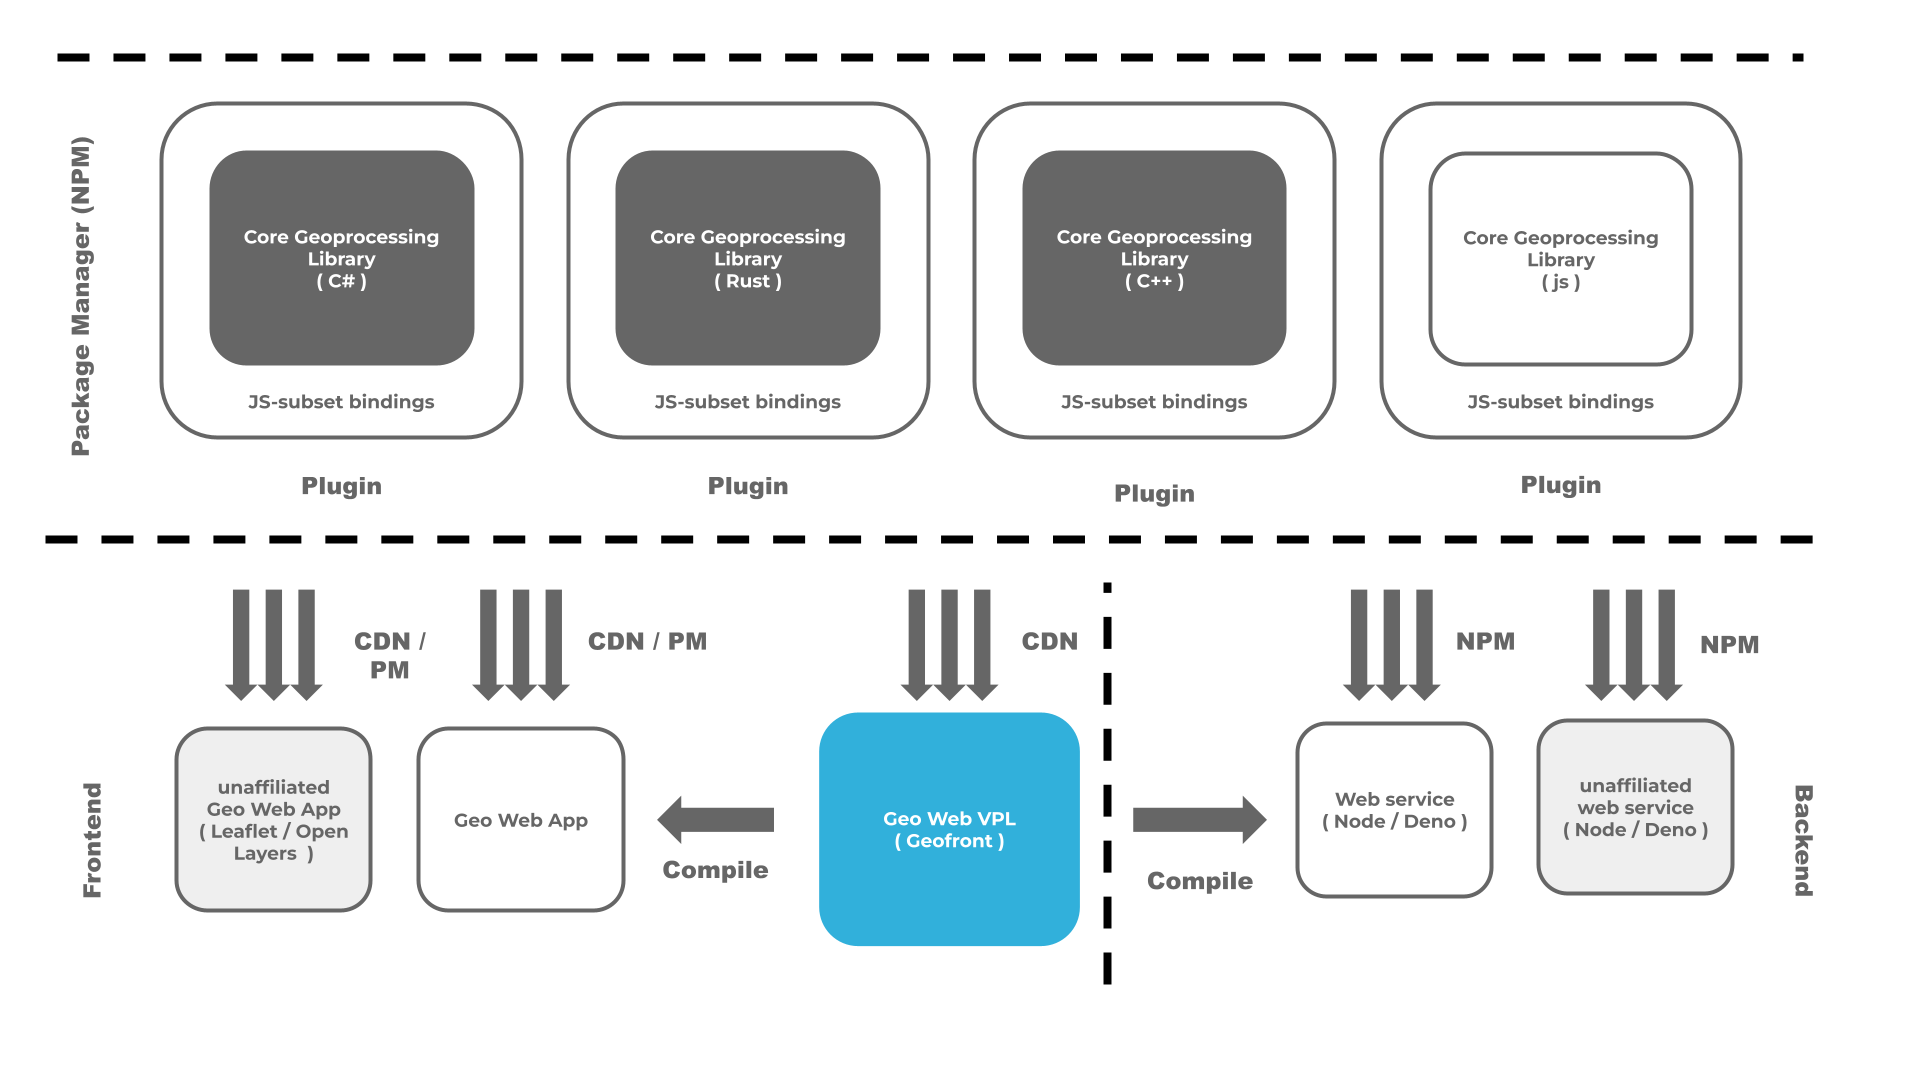
\includegraphics[width=340px]{Model Proposal.png}
  \caption{Plugin Model}
  \label{fig:plugin-model}
\end{figure}

The library model consists of two components: the design for a geo-web-vpl library, and the design for a 
loader on the side of the VPL. 
The central idea for this model is to take the wasm-wrappers created in \refsec{sec:method-two}, and to either interpret the required information from the wasm binary and related files, or, if that is impossible, add the required information in the wasm wrapper library itself.
By doing so, we make sure that at the very least, only one wrapper library is required for exposing any non-js library to the \ac{geo-web-vpl}.
The following information is required for the VPL to load a geocomputation library, and convert it into visual components:

Mandatory: 
\begin{enumerate}[-]
  \item A list of all functions present in the library, named.
  \item A list of all custom types (structs / classes) present in the library, also named.
  \item Per function:  
  \subitem A list of all input parameters, name and type.
  \subitem An output type.
\end{enumerate}

Optional: 
\begin{enumerate}[-]
  \item Per function:
  \subitem A custom name.
  \subitem A description to explain usage.

  \item Per type:
  \subitem A custom name.
  \subitem A description to explain usage.
  \subitem A definition of how to serialize and deserialize this type  
  \subitem A definition of how to render this type in 3D
  \subitem A definition of how to convert this type to basic types present within the geo-web-vpl.  
\end{enumerate}

The necessity to automate loading geocomputation libraries means that the \ac{geo-web-vpl} needs to be able to extract this information automatically. 
For scope reasons, the study limits itself to only interpret the \textbf{mandatory} information fully automatically. 
This can be achieved by using the Rust-wasm toolset "\m{wasm-bindgen}". 
\m{wasm-bindgen} is able to generate javascript wrapper bindings for a \ac{wasm} library, accompanied by TypeScript type definitions (Source). 
These are given in a 'd.ts' file, which can be understood as a header file, exposing the types required by all functions found in its corresponding javascript file. 
By including the typescript compiler in the \ac{geo-web-vpl} prototype, this header file can be loaded and interpreted to find all mandatory data, including the names and path of functions and types. 
These can then be accessed by reflecting these names and paths with the javascript files, which in turn calls the underlying \ac{wasm} binary.

The \textbf{optional} data is exposed by using 'magic methods', a strategy influenced by the python programming language (source). 
The library loader of the VPL will load certain functions, types, and methods in a special way, indicated by a naming convention. 
These functions are loaded by the vpl, but will not be converted into visual components. 
Instead, these functions are programmatically called when the VPL engine or the user requires this optional aspect. 

%%%%%%%%%%%%%%%%%%%%%%%%%%%%%%%%%%%%%%%%%%%%%%%%%%%%%%%%%%%%%%%%%%%%%%%%%%%%%%%
%%%%%%%%%%%%%%%%%%%%%%%%%%%%%%%%%%%%%%%%%%%%%%%%%%%%%%%%%%%%%%%%%%%%%%%%%%%%%%%
%%%%%%%%%%%%%%%%%%%%%%%%%%%%%%%%%%%%%%%%%%%%%%%%%%%%%%%%%%%%%%%%%%%%%%%%%%%%%%%
%%%%%%%%%%%%%%%%%%%%%%%%%%%%%%%%%%%%%%%%%%%%%%%%%%%%%%%%%%%%%%%%%%%%%%%%%%%%%%%
%%%%%%%%%%%%%%%%%%%%%%%%%%%%%%%%%%%%%%%%%%%%%%%%%%%%%%%%%%%%%%%%%%%%%%%%%%%%%%%

\section{\mySubRQFourTitle} 
\label{sec:method-four}

The final component of the methodology is dedicated to overcoming the fourth and final challenge to realizing a \ac{geo-web-vpl}, and involves the utilization of all aforementioned components. 
In this section, we wish to discover the practical usefulness of a \ac{geo-web-vpl}, encompassed by the research question : \mySubRQFour

% What are the advantages and disadvantages of using an existing geoprocessing library through a geo-web-vpl, as opposed to native utilization of said library?

\subsection*{Why}
This component of the methodology is included in the study because of the following: 
It might be the case that a geo-web-vpl \emph{is} able to be interfaced using a web-browser, and \emph{is} able to load and run functions from native, non-js geo-computation libraries. 
And still, it might not be able to successfully \emph{use} these libraries. 
The entire idea of a vpl might not be sensible for the operation at hand, or some other, unforeseen aspects mitigates the practical usefulness of the environment. 
It is therefore vital to access the actual usage of the application for accessing a geocomputation library.

\subsection*{How}
To answer the question of \mySubRQFourTitle, the following plan was used: 
\begin{enumerate}[-]
  \item Develop a representative use-case application within the prototype \ac{geo-web-vpl}.
  \item Develop a command line application capable of the very same process.
  \item Assess both applications according to a series of assessment questions.
\end{enumerate}

The execution of this component of the methodology is found in \refchap{chap:experiments}.

\subsection{use-case application}
The application used in both test cases is an "isocurves from DTM" process. 
But also: we want the iso-curves of a specific location. How to get this data is part of the exercise

\begin{note}
- This is subject to change, according to how much I can accomplish 

- find the required height data as WFS / WMS
- determine a boundary
- load a dtm as a regular png / tiff image
- specify the parameters, like height delta, smoothness.
- marching squares
- post-process curves
- save as wkt, geojson, or some other well-known vector format


\end{note}

\subsection{Assessment Criteria}

\begin{note}
Just ideas:

  - how to get the data you need? 
  - how to extract the part that you need?
  - how to specify the input data to the application? 
  - how to get the height parameter 'just right'? 
  
It is not about the application, is it about DOING the desired geocomputation.  

NOTE: you might want to connect this to the 3.2.1 experiment.

\end{note}
  

